\documentclass[14pt, a4paper]{article}

\usepackage[utf8]{inputenc}
\usepackage[T2A]{fontenc}

\usepackage{graphicx}
\graphicspath{ {images/} }

\tolerance 1414
\hbadness 1414
\emergencystretch 1.5em
\hfuzz 0.3pt        % размер максимального переполнения без warning'a
\widowpenalty=10000 % запрещает одиночную строку абзаца в начале страницы 
\vfuzz \hfuzz
\raggedbottom       % если на странице мало содержимого, добавить пустое место в конце, а не в середине страницы

\title{ЛАБОРАТОРНАЯ РАБОТА №1
ИЗМЕРЕНИЕ ЭЛЕКТРИЧЕСКИХ ВЕЛИЧИН И ПАРАМЕТРОВ
ЭЛЕМЕНТОВ ЭЛЕКТРИЧЕСКИХ ЦЕПЕЙ
}
\author{Новоженов П.А. ЭН-26}
\date{}

\begin{document}

    \maketitle

    \thispagestyle{empty}

    \clearpage

    \section*{Цели работы}

    \begin{enumerate}
    \item Ознакомиться с измерительными приборами, 
    источниками питания и основными элементами 
    программной среды Multisim.
    \item  Изучить методы и приобрести навыки 
    измерения основных параметров электрических цепей, 
    ознакомиться c свойствами индуктивных катушек и
    конденсаторов в цепях постоянного тока, рассчитать параметры и построить делители напряжения и тока.
    \end{enumerate}

    \section*{Перечень использованных приборов}
    \begin{itemize}
        \item Резистор
        \item Ключ 
        \item Мультиметр XMM
        \item Амперметр
        \item Вольтметр
        \item Источник тока
        \item Источник напряжения
        \item Катушка индуктивности
        \item Конденсатор
    \end{itemize}

    \clearpage

    \section*{Задание 1 Измерение сопротивлений}

    {
        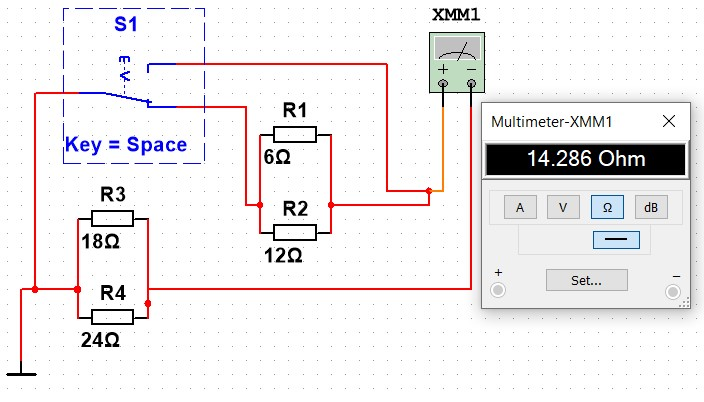
\includegraphics[width=0.8\textwidth]{1lab1.1.jpg}
        \centering
    }

    Найдем сопротивления $R_{12}$, $R_{34}$ и $R_{1234}$:
    $$R_{12} = \frac{R_1R_2}{R_1+R_2} = \frac{6*12}{6+12} = \frac{72}{18} = 4 \Omega$$
    $$R_{34} = \frac{R_3R_4}{R_3+R_4} = \frac{18*24}{18+24} = \frac{432}{42} = 10.286 \Omega$$
    $$R_{1234} = R_{12} + R_{34} = 4 + 10.286 = 14.286 \Omega$$

    {
        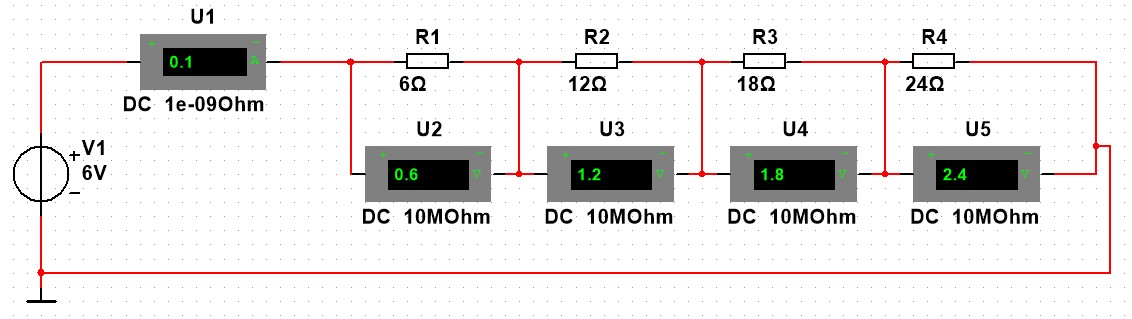
\includegraphics[width=0.8\textwidth]{1lab1.2.jpg}
        \centering
    }


    На схеме амперметр показывает значение тока в цепи, 
    вольтметры показывают напряжение на каждом из резисторов. 
    Найдем сопротивление каждого резистора по формуле:
    $$R = \frac{U}{I}$$
    $$R_1 = \frac{0.6}{0.1} = 6 \Omega$$
    $$R_2 = \frac{1.2}{0.1} = 12 \Omega$$
    $$R_3 = \frac{1.8}{0.1} = 18 \Omega$$
    $$R_4 = \frac{2.4}{0.1} = 24 \Omega$$

    {
        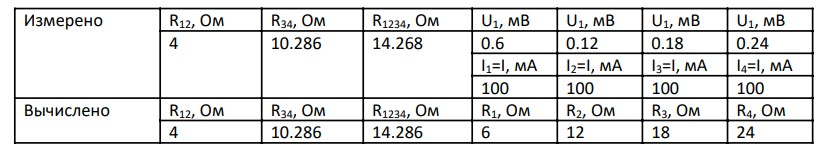
\includegraphics[width=\textwidth]{table1.jpg}
        \centering
    }


    \section*{Задание 2 Реактивные элементы в цепях постоянного тока}

    На схеме 2.1 видно, что напряжение
    на катушке очень мало,
    значит идельная катушка индуктивности не имеет сопротивления.

    {
        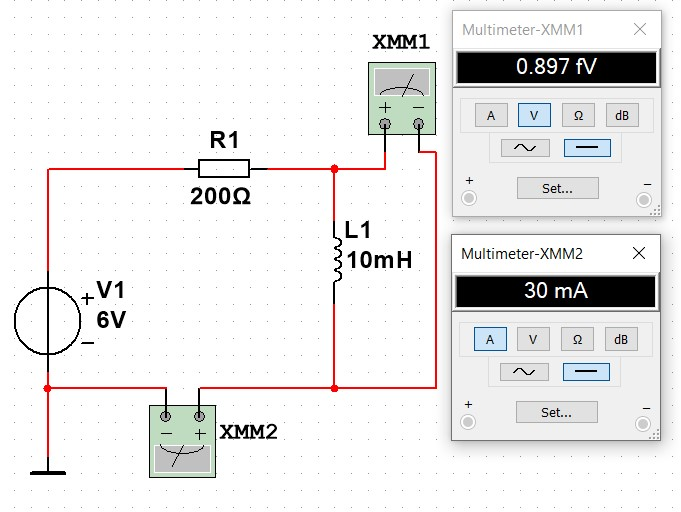
\includegraphics[width=0.8\textwidth]{1lab2.1.jpg}
        \centering
    }

    На схеме 2.2 видно, что постоянный ток через конденсатор не течет.
    Конденсатор в цепи постоянного тока является разрывом цепи.

    {
        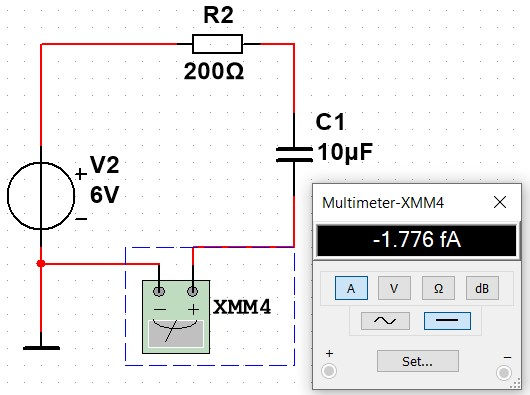
\includegraphics[width=0.8\textwidth]{1lab2.2.jpg}
        \centering
    }

    \clearpage


    \section*{Задание 3 Делитель напряжения}

    {
        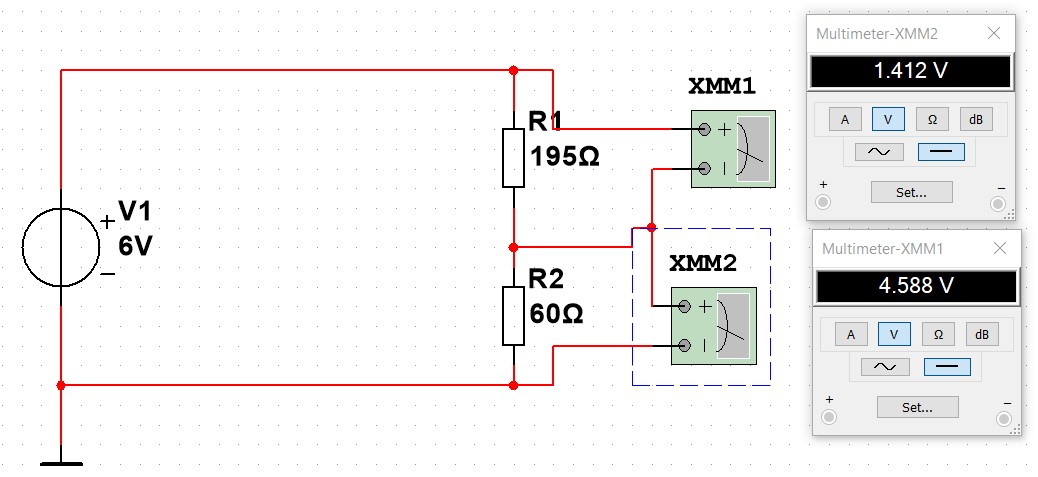
\includegraphics[width=0.8\textwidth]{1lab3.jpg}
        \centering
    }

    Рассчитаем характеристики делителя напряжения:
    $$I = \frac{E}{R_1 + R_2} = \frac{6}{195+60} = 0.0235$$
    $$U_1 = IR_1 = 0.0235 * 195 = 4.589 V$$
    $$U_2 = IR_2 = 0.0235 * 6 = 1.412 V$$

    \section*{Задание 4 Делитель тока}
    
    {
        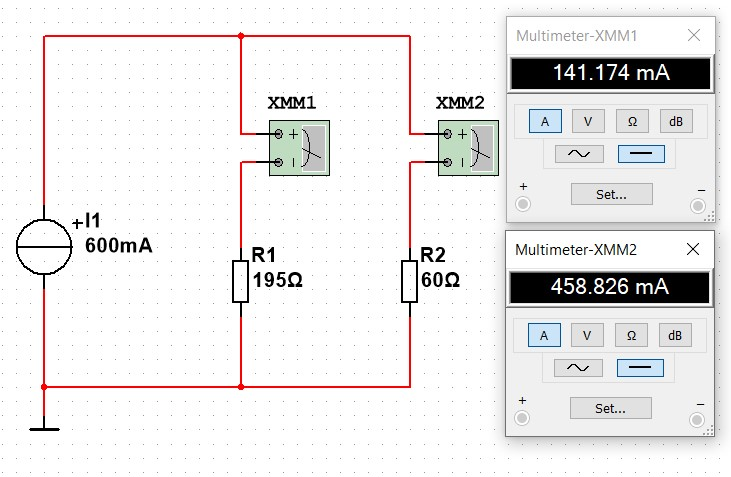
\includegraphics[width=0.8\textwidth]{1lab4.jpg}
        \centering
    }

    Рассчитаем значения токов:
    $$I_1 = I\frac{R_1}{R_1 + R_2} = 0.6 \frac{195}{195 + 60} = 0.459 A$$
    $$I_2 = I\frac{R_2}{R_1 + R_2} = 0.6 \frac{60}{195 + 60} = 0.141 A$$

    \clearpage


    \section*{Выводы}

    %   Ознакомиться с измерительными приборами, источниками питания и основными элементами программной среды Multisim.
    %   Изучить методы и приобрести навыки измерения основных параметров электрических цепей, 
    % ознакомиться c свойствами индуктивных катушек иконденсаторов в цепях постоянного тока, рассчитать параметры и построить делители напряжения и тока.
    

    В ходе выполнения работы я ознакомился с измерительными приборами, 
    источниками питания и основными элементами среды Multisim. 
    А также изучил методы и приобрел навыки измерения основных параметров электрических цепей,
    ознакомился с свойствами индуктивных катушек и конденсаторов в цепях постоянного,
    рассчитал пареметры и построил делители тока и напряжения.

\end{document}

